\chapter{Implementazione}
Il seguente capitolo motiva e dettaglia le scelte implementative ritenute rilevanti per una corretta comprensione del progetto. È bene precisare che nel codice è presente la Scaladoc che permette di dettagliare ogni singola parte del codice.

\section{Utilizzo del paradigma funzionale}
Sin dalle prime fasi di progettazione il team ha intrapreso la scelta di utilizzare il più possibile il paradigma funzionale, cercando di non ricorrere alle usuali abitudini di programmazione object-oriented. Per fare ciò sono state utilizzate diverse metodologie: 
\begin{itemize}
    \item inutilizzo dei side effect, creando ad ogni modifica un nuovo ogetto immutabile.
    \item utilizzo di funzioni ricorsive.
    \item utilizzo di funzioni higher-order che permettono una facile ed immediata realizzazione del parttern Strategy, consentono una maggiore riutilizzabilità del codice. In questo modo è possibile passare alle funzioni strategie esterne, non necessitando così di modificare il codice.
\end{itemize}

Rispettando quanto sopra elencato, il Controller e il Model dell'applicazione sono stati realizzati con un approccio puramente funzionale. La View adottare anch'essa il paradigma descritto in questo corso attraverso l'utilizzo della libreria cats.effect.IO.

\subsection{Model}

Come anticipato nella sezione precedente ogni entità che entra a far parte della simulazione deve soddisfare il requisito di essere del tipo SimulableEntity. Tale classe racchiude di ogni entità struttura e comportamento, come descritto dalla Figura \ref{fig:simentity}. 


\begin{figure}[h!]
\centering
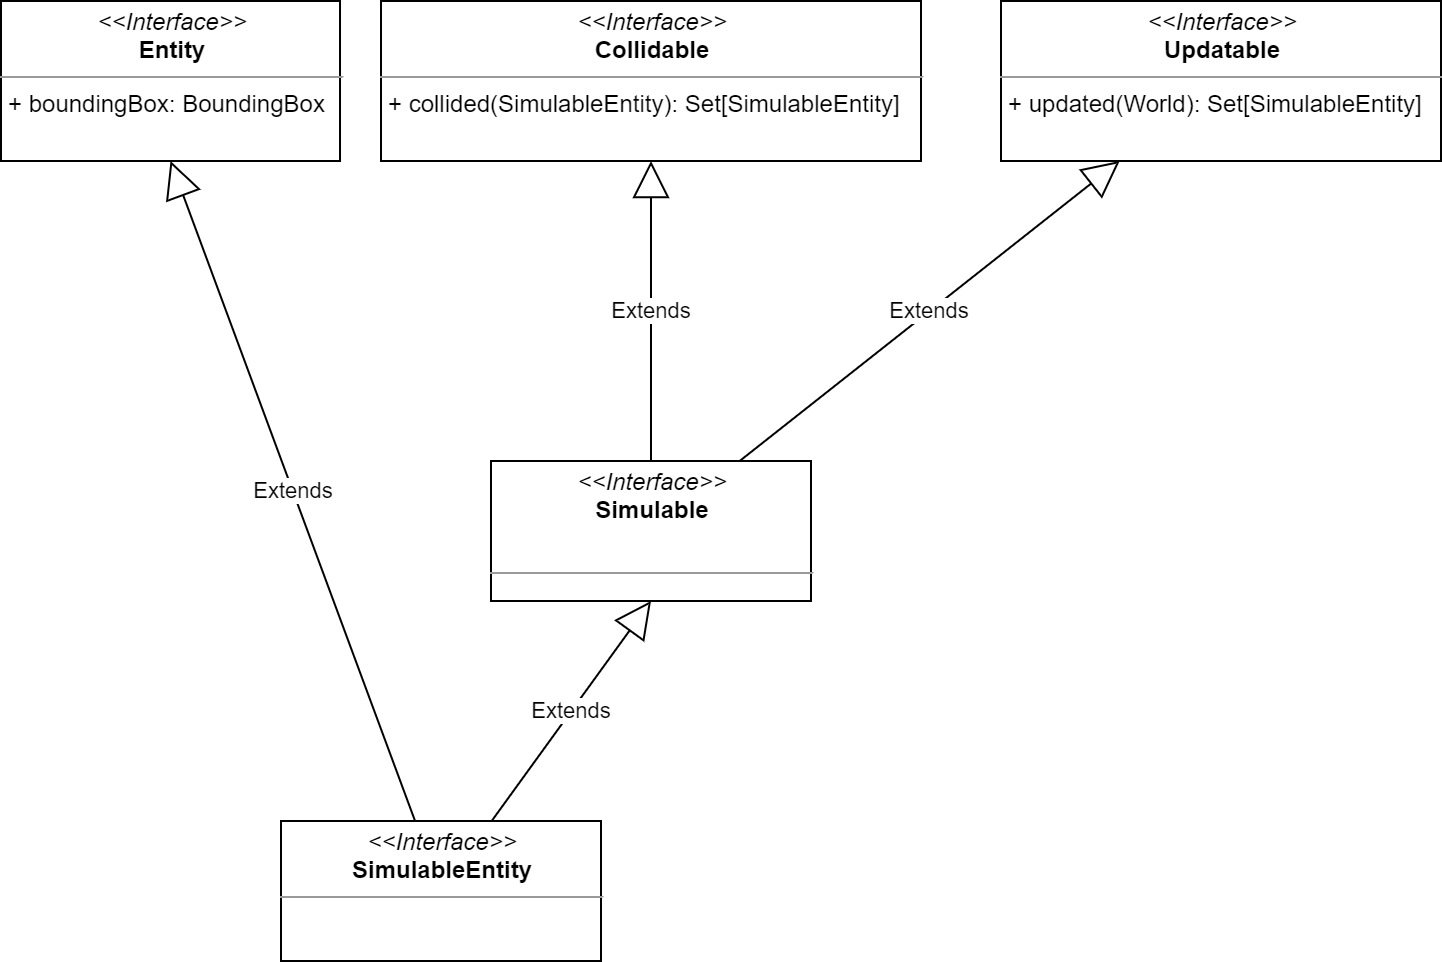
\includegraphics[width=\textwidth, scale=0.44]{img/SimulableEntity.png}
\caption{Simulable Entity UML}
\label{fig:simentity}
\end{figure}

Per l'implementazione del comportamento di un'entità, quindi l'implementazione delle interfaccie \code{Updatable} e \code{Collidable}, ove necessario definire un comportamento differente dal \code{NeutralBehaviour}, si è fatto uso dei self types. Tale pattern di programmazione è un modo per dichiarare che un trait deve essere mescolato con mixin in un altro trait, anche se non lo estende direttamente. Questa tecnica permette sostanzialmente di fare dependency injection dichiarando esplicitamente nel trait le dipendenze di cui un componente necessita.

Uno dei vantaggi di separare comportamento da struttura è quello della riusabilità dei concetti e quindi del codice. Andando quindi a mescolare strutture e comportamenti è possibile combinarli e riutilizzarli per estensioni  e implementazioni future. 

Prendendo come esempio l'implementazione della Figura \ref{fig:Blob implementation} il \code{BaseBlob}, questa classe estende dal trait Blob (tale trait è un'interfaccia \code{mixin}, viene utilizzato quindi il polimorfismo ad hoc). Il trait blob ne definisce la struttura mentre il comportamento è definito nel trait \code{BaseBlobBehaviour}. Il comportamento del \code{CannibalBlob}, pur mantenedo la struttura dati derivata dal \code{Blob}, è derivato da \code{CannibalBlobBehaviour}

\begin{figure}[h!]
\centering
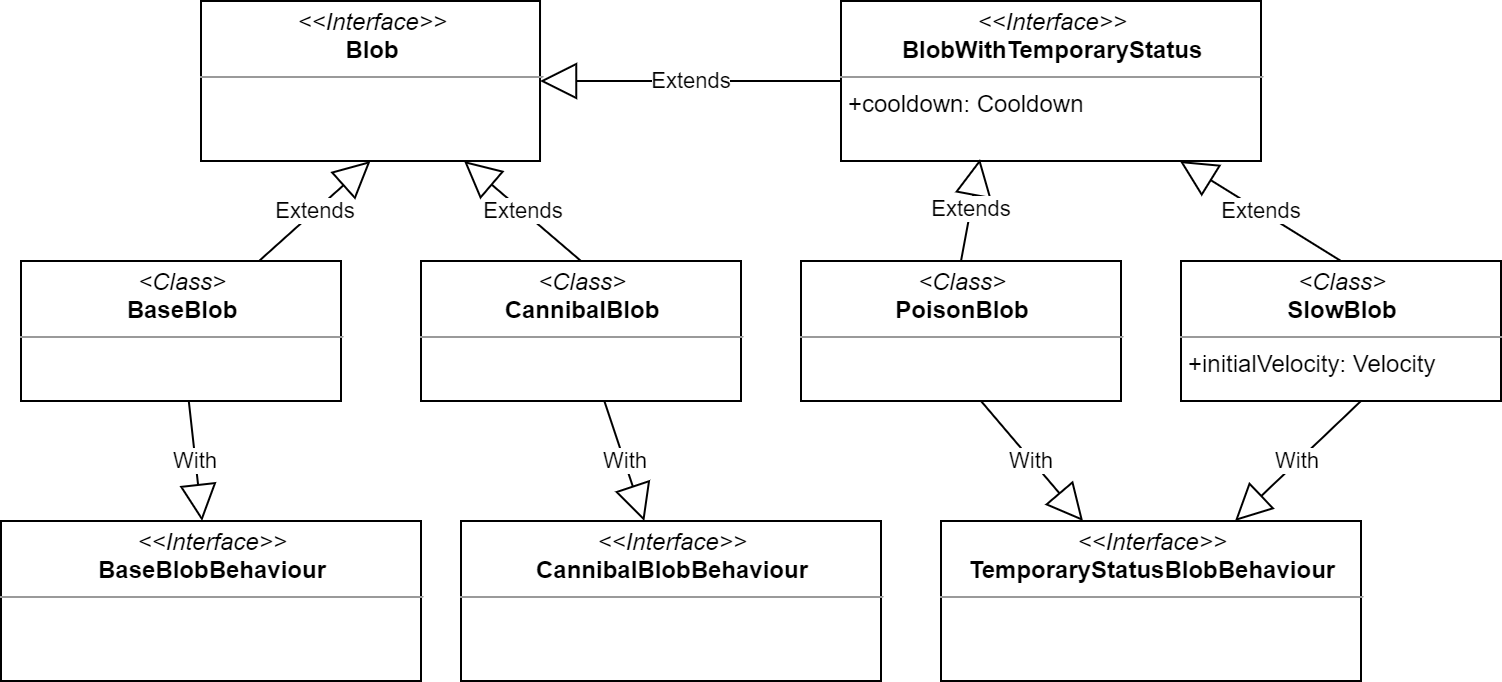
\includegraphics[width=\textwidth, scale=0.44]{img/Blob implementation.png}
\caption{Blob implementation hierarchy  UML}
\label{fig:Blob implementation}
\end{figure}


\subsection{View}
Bisogna parlare della View, in particolare dell'approccio funzionale utilizzato.


\subsection{Stream e World}
Il World è stato modellato come un contenitore immutabile delle proprietà della simulazione e delle entità che vi partecipano. Al fine di memorizzare i dati necessari ai fini di analisi, esso è definito in termini di se stesso: worldHistory è uno stream costituito dalle istanze di World riferite alle iterazioni precedenti. La lazy evaluation degli stream permette di non appesantire la computazione del simulationLoop con un carico di lavoro altrimenti insostenibile: impiegare una collezione non lazy come una lista avrebbe comportato la creazione di una moltitudine di strutture dati intermedie di grandissime dimensioni. 

\begin{figure}[h!]
\centering
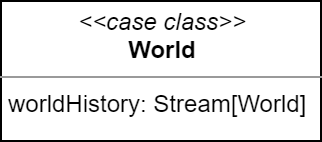
\includegraphics[scale=0.30]{img/WorldDetail.png}
\caption{Dettaglio di worldHistory come Stream per la memorizzazione delle informazioni sugli World alle iterazioni passate necessarie alla elaborazione statistica finale}
\label{fig:worldDetail}
\end{figure}

Grazie agli stream, la valutazione della grande quantità di dati accumulata avviene solo alla conclusione della simulazione e al momento del processamento dei dati a fini statistici, non interferendo così con l’andamento della simulazione.

\subsection{Currying e partial application}
Per incentivare il riuso, applicare il principio DRY, agevolarne l’eventuale futuro utilizzo come parametro higher order e gestire meglio l’alto numero di parametri, la funzione sinusoidal è stata implementata come funzione curried e le sue più comuni configurazioni (utilizzate più volte nel codice) sono state tramutate in partially-applied function (zeroPhasedinusoidal, zeroPhasedZeroYTranslatedSinusoidal etc). È stato utilizzato il currying anche nel codice di visualizzazione dei parametri (indicatorsUpdated di SwingView) per evitare duplicazioni ed accomunare invocazioni multiple sotto la stessa signature, indipendente da quella originale.

\subsection{Memoizing}
Dato l’andamento periodico di temperatura e di luminosità del World, le cui curve sinusoidali esprimono ciascuna gli stessi valori negli stessi momenti di giornate diverse, e data la complessità computazionale del calcolo trigonometrico (rispetto alla aritmetica intera ad es.), è stato applicato il pattern flyweight con memoization di valori di luminosità, temperatura e variazione della proprietà “campo visivo” (dell’astrazione Intelligent) rispetto alla luminosità. Al termine della prima giornata di simulazione, tali valori saranno già stati computati e nelle successive iterazioni sarà sufficiente reperirli con accesso costante.

\section{Paradigma logico}
Dopo un'accurata e dettagliata analisi della logica di movimento delle entità, il team si era proposto di integrare nel progetto il paradigma logico. Ciò è avvenuto attraverso la libreria TuProlog. In particolare, la logica di movimento ideata e implementata è la seguente:
\begin{itemize}
    \item nel caso in cui nessuna entità commestibile sia presente all'interno del campo visivo, l'entità in considerazione deve muoversi in una direzione casuale.
    \item nel caso in cui una o più entità commestibili siano presenti all'interno del campo visivo, l'entità dovrà dirigersi verso il nutrimento più vicino.
\end{itemize}
La teoria Prolog presente nel file \code{src/main/resources/movementTheory.pl} consente di ricercare la presenza di un entità commestibile all'interno del campo visivo tra tutte le entità presenti nella simulazione, ed agire di conseguenza nel caso in cui l'entità sia presente o meno all'interno del campo visivo. Tuttavia per problemi legati alle performance (in quanto non possibile rispettare il requisito 4.1) si è adottato un approccio ibrido, in cui la ricerca di un entità all'interno del campo visivo viene effettuata con il paradigma funzionale, lasciando poi il calcolo della nuova posizione al paradigma logico.

\section{Test}
La realizzazione di test è stato un aspetto fondamentale per verificare la correttezza e la qualità del codice, garantendo anche un'ulteriore documentazione del software sviluppato. La loro implementazione non è avvenuta con la metodologia stringente del Test Driven Development (TDD), bensì con un approccio più tradizionale, in cui la funzionalità veniva testata una volta pronta. In particolare è stata utilizzata la libreria ScalaTest, mantenendo uno stile omogeneo utilizzando \textbf{FunSpec}. L'impiego di \textbf{Travis CI} ha comunque permesso di verificare che eventuali modifiche al codice non infierissero negativamente sul comportamento atteso delle funzioni senza dover costantemente tenere d'occhio i test manualmente.

\section{Suddivisione del lavoro}
Inizialmente il team ha effettuato un analisi preliminare, dettagliando quali caratteristiche e requisti il software dovesse esibire. In seguito a ciò, si sono susseguiti una frequente serie di meeting (in cui era presente tutto il team) dove, partendo da piccoli diagrammi UML che descrivevano a grandi linee l'architettura del sistema, si è scesi sempre più in dettaglio fino a creare l'intero design architetturale. È bene precisare che il design architetturale è stato ideato in ciascuna sua parte da tutto il team, in modo coeso e collaborativo. Successivamente, in seguito alla realizzazione di un design architetturale dettagliato per ogni funzionalità del software, a ciascun membro del team è stata assegnata una parte dello sviluppo. Nel dettaglio:

\subsection{Rei Beshiri}
Il mio ruolo nel progetto dal punto di vista implementativo riguarda principalmente la realizzazione e la manutenzione delle entità del modello, seguendone lo sviluppo dalla prima implementazione, e delle sue diverse componenti in collaborazione con i membri del team, in particolare delle entità blob del loro comportamento e reazione con l'ambiente circostante e alle intersezioni tra le varie entità in gioco, degli effetti delle stesse così come della loro bounding box.
Ogni qual volta risultasse necessario dal team apportare modifiche anche pesanti al codice non mi sono fatto problemi ad applicarle, anzi è spesso risultato semplice attuare azioni di manutenzione correttiva o evolutiva al codice, segno di un buon lavoro di design.

I test sviluppati riguardano le classi:
\begin{itemize}
    \item \code{BlobTest}
    \item \code{DegradationTest}
    \item \code{IntersectionTest}
\end{itemize}

\subsection{Andrea Betti}
Ho contribuito insieme a Rei Beshiri all'implementazione dei comportamenti delle diverse entità della simulazione in \code{evo\_sim.model.EntityBehaviour} e agli effetti applicabili dalle entità \textit{Effectful} in \code{evo\_sim.model.effects.CollisionEffect}, realizzando le classi e le funzioni relative alle entità \textit{Food} e \textit{Plant} e contribuendo in misura minore ai comportamenti delle entità \textit{Blob} e all'estensione di \code{evo\_sim.model.EntityStructure}.

Ho inoltre implementato la logica di rappresentazione della simulazione utilizzando \texttt{Swing} all'interno della classe \code{evo\_sim.view.swing.custom.components.ShapesPanel}, utilizzata nella funzione \code{rendered} di \code{evo\_sim.view.swing.SwingView} realizzata da Alessandro Oliva.

Per quanto riguarda i test, ho realizzato \code{FoodTests} e \code{PlantTests}.

\subsection{Daniele Giulianini}

\subsection{Alessandro Oliva}
Il mio contributo nel model è consistito nello sviluppo delle entità \textit{Obstacle}, le entità con status temporanei (il cui raffinamento è però stato curato da Rei Beshiri), in particolare lo \textit{SlowBlob}.

Mi sono occupato inoltre del ciclo giorno notte della simulazione, con rispettiva influenza sui blob in termini di velocità e campo visivo tramite appositi moduli di funzioni.

Per quanto riguarda la View, ne ho seguito lo sviluppo dalla prima versione in \texttt{ScalaFX} fino all'implementazione puramente funzionale attraverso il framework \texttt{Cats}, del quale con l'importante contributo di Daniele Giulianini è stato sviluppato un intero package che permette di utilizzare componenti Swing in maniera funzionale. Sempre con Daniele Giulianini mi sono occupato dell'integrazione fra View e Core mediante il framework monadico. Parallelamente a questa versione è stata sviluppata un interfaccia a linea di comando per permettere la fruizione dell'applicazione nella sua interezza anche mentre si lavorava alla View.

I test da me sviluppati sono inclusi in \code{ObstacleTests}.

\subsubsection{Andrea Vaienti}
Sono principalmente due le porzioni del progetto di cui mi sono occupato: 

\begin{itemize}
    \item l'intelligenza artificiale che consente il movimento delle entità all'interno del mondo
    \item statistiche finali, dal loro calcolo fino alla creazione e renderizzazione dei grafici che le visualizzano.
\end{itemize}

Per quanto riguarda il movimento, come anticipato precedentemente, la logica era stata inizialmente implementata in Scala (\code{DemonstrationCompletelyScalaMovement}). Successivamente, dopo aver effettuato controlli su una possibile implementazione attraverso il paradigma logico, è stata realizzata in Prolog (\code{DemonstrationCompletelyPrologMovement}). Infine, a causa dei problemi di performance sopraindicati è stata utilizzata una soluzione ibrida (Scala + Prolog), presente nel file \code{MovingStrategies}. Tutte queste tre soluzioni sono state opportunamente testate in \code{MovementTests}. Per la visualizzazione delle statiche finale, prima di tutto è stata effettuata un'esplorazione delle possibili librerie che permettessero la visualizzazione dei grafici all'interno dell'interfaccia grafica, che si è conclusa con la scelta di utilizzare \hyperlink{https://knowm.org/open-source/xchart/}{XChart}. In seguito a ciò è stato realizzato un ChartBuilder, che consente attraverso appositi parametri di creare 3 tipologie di grafici. Così facendo, qualsiasi membro del Team o futuro sviluppatore, potrebbe costruire e successivamente visualizzare un grafico contenente i propri valori. Il calcolo delle statistiche finali è stato implementato nel file \code{FinalStats}, in cui si è fatto ampiamente uso di funzioni higher-order per consentire una maggiore riutilizzabilità del codice. Per precisione, vengono di seguito elencati i package contententi le implementazioni da me svolte:

\begin{itemize}
    \item \texttt{model.entities.entityStructure.movement}
    \item \texttt{prolog}
    \item \texttt{view.swing.chart}
    \item \texttt{model.world.dataProcessing}
\end{itemize}